% Styles til elementer
\tikzstyle{ledningsband} 	=	[rectangle, draw, thick, text width=10em, text centered, minimum height=4em]
\tikzstyle{valensband} 		= [rectangle, draw, thick, text width=10em, text centered, minimum height=4em]

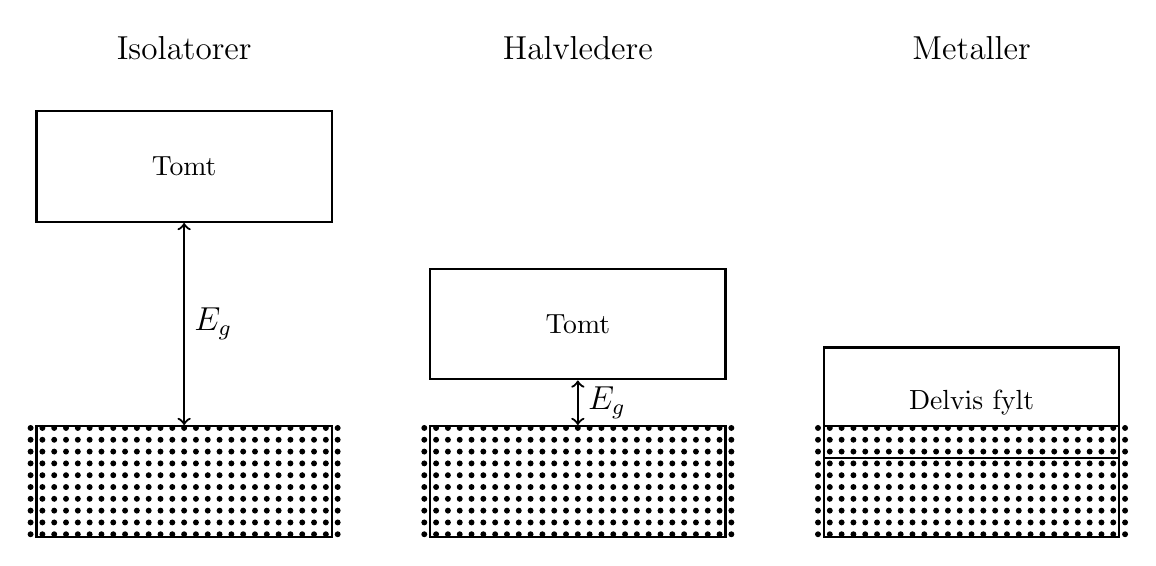
\begin{tikzpicture}

	% Boksene i bunnen
	\node[valensband]	(valens_isolator)																										{};
	\node[valensband]	(valens_halvleder)	[right of=valens_isolator,  node distance=5cm]	{};
	\node[valensband]	(valens_metall)			[right of=valens_halvleder, node distance=5cm]	{};	
	
	% Boksene i toppen
	\node[ledningsband]	(lednings_isolator)		[above of=valens_isolator, 	node distance=4cm]	{Tomt};
	\node[ledningsband]	(lednings_halvleder)	[above of=valens_halvleder, node distance=2cm]	{Tomt};
	\node[ledningsband]	(lednings_metall)			[above of=valens_metall, 		node distance=1cm]	{Delvis fylt};
	
	% Piler
	\draw[thick,<->] (valens_isolator)  -- node[right] {\large $E_g$} (lednings_isolator);
	\draw[thick,<->] (valens_halvleder) -- node[right] {\large $E_g$} (lednings_halvleder);
	
	% Tekst p� toppen
	\node (isolator_tekst)  [above of=lednings_isolator,node distance=1.5cm]	{\large Isolatorer};
	\node (halvleder_tekst) [right of=isolator_tekst, 	node distance=5cm] 		{\large Halvledere};
	\node (metaller_tekst)  [right of=halvleder_tekst, 	node distance=5cm] 		{\large Metaller};
	
	% Elektroner i valensb�nd
	\foreach \y in {0,0.15,...,1.4}
		\foreach \x in {0,0.15,...,4} {
			\draw (\x-1.95,\y-0.67) circle (0.03cm) [fill=black];	% Isolator
			\draw (\x+3.05,\y-0.67) circle (0.03cm) [fill=black];	% Halvleder
			\draw (\x+8.05,\y-0.67) circle (0.03cm) [fill=black];	% Metall
		}	
	
\end{tikzpicture}	

